\documentclass[11pt, a4paper]{article}
\usepackage{pdfpages}
\usepackage{parallel}
\usepackage[T2A]{fontenc}
\usepackage{ucs}
\usepackage[utf8x]{inputenc}
\usepackage[polish,english,russian]{babel}
\usepackage{hyperref}
\usepackage{rotating}
\usepackage[inner=2cm,top=1.8cm,outer=2cm,bottom=2.3cm,nohead]{geometry}
\usepackage{listings}
\usepackage{graphicx}
\usepackage{wrapfig}
\usepackage{longtable}
\usepackage{indentfirst}
\usepackage{array}
\usepackage{tikzsymbols}
\usepackage{soul}
\usepackage[ruled,vlined]{algorithm2e}
%\counterwithout{figure}{section} 

\usepackage{url}
\makeatletter
\g@addto@macro{\UrlBreaks}{\UrlOrds}
\makeatother

\newcolumntype{P}[1]{>{\raggedright\arraybackslash}p{#1}}
\frenchspacing
\usepackage{fixltx2e} %text sub- and superscripts
\usepackage{icomma} % коскі ў матэматычным рэжыме
\PreloadUnicodePage{4}

\newcommand{\longpage}{\enlargethispage{\baselineskip}}
\newcommand{\shortpage}{\enlargethispage{-\baselineskip}}

\def\switchlang#1{\expandafter\csname switchlang#1\endcsname}
\def\switchlangbe{
\let\saverefname=\refname%
\def\refname{Літаратура}%
\def\figurename{Іл.}%
}
\def\switchlangen{
\let\saverefname=\refname%
\def\refname{References}%
\def\figurename{Fig.}%
}
\def\switchlangru{
\let\saverefname=\refname%
\let\savefigurename=\figurename%
\def\refname{Литература}%
\def\figurename{Рис.}%
}

\hyphenation{admi-ni-stra-tive}
\hyphenation{ex-pe-ri-ence}
\hyphenation{fle-xi-bi-li-ty}
\hyphenation{Py-thon}
\hyphenation{ma-the-ma-ti-cal}
\hyphenation{re-ported}
\hyphenation{imp-le-menta-tions}
\hyphenation{pro-vides}
\hyphenation{en-gi-neering}
\hyphenation{com-pa-ti-bi-li-ty}
\hyphenation{im-pos-sible}
\hyphenation{desk-top}
\hyphenation{elec-tro-nic}
\hyphenation{com-pa-ny}
\hyphenation{de-ve-lop-ment}
\hyphenation{de-ve-loping}
\hyphenation{de-ve-lop}
\hyphenation{da-ta-ba-se}
\hyphenation{plat-forms}
\hyphenation{or-ga-ni-za-tion}
\hyphenation{pro-gramming}
\hyphenation{in-stru-ments}
\hyphenation{Li-nux}
\hyphenation{sour-ce}
\hyphenation{en-vi-ron-ment}
\hyphenation{Te-le-pathy}
\hyphenation{Li-nux-ov-ka}
\hyphenation{Open-BSD}
\hyphenation{Free-BSD}
\hyphenation{men-ti-on-ed}
\hyphenation{app-li-ca-tion}

\def\progref!#1!{\texttt{#1}}
\renewcommand{\arraystretch}{2} %Іначай формулы ў матрыцы зліпаюцца з лініямі
\usepackage{array}

\def\interview #1 (#2), #3, #4, #5\par{

\section[#1, #3, #4]{#1 -- #3, #4}
\def\qname{LVEE}
\def\aname{#1}
\def\q ##1\par{{\noindent \bf \qname: ##1 }\par}
\def\a{{\noindent \bf \aname: } \def\qname{L}\def\aname{#2}}
}

\def\interview* #1 (#2), #3, #4, #5\par{

\section*{#1\\{\small\rm #3, #4. #5}}
\ifx\ParallelWhichBox\undefined%
    \addcontentsline{toc}{section}{#1, #3, #4}%
\else%
\ifnum\ParallelWhichBox=0%
    \addcontentsline{toc}{section}{#1, #3, #4}%
\fi\fi%

\def\qname{LVEE}
\def\aname{#1}
\def\q ##1\par{{\noindent \bf \qname: ##1 }\par}
\def\a{{\noindent \bf \aname: } \def\qname{L}\def\aname{#2}}
}

\newcommand{\interviewfooter}[1]{
\vskip 1em
\noindent \textit{#1}
}

\switchlang{en}
\begin{document}

\title{1986 "--- NEC Crystal mouse}
\date{}
\maketitle
\selectlanguage{english}
In September 1986, NEC Corporation announced the EWS 4800 UNIX workstation. This computer was designed as a workstation for engineers to improve the efficiency of solving problems such as software development, computer-aided design, scientific and engineering calculations, and the collection and analysis of experimental data \cite{yt}. The computer was equipped with a graphical multi-window interface and a large 20-inch $1280 \times 1024 \times 256$ display. This powerful workstation came with the NEC Crystal Mouse (figure \ref{fig:NECCrystalPic}).

\begin{figure}[h]
    \centering
    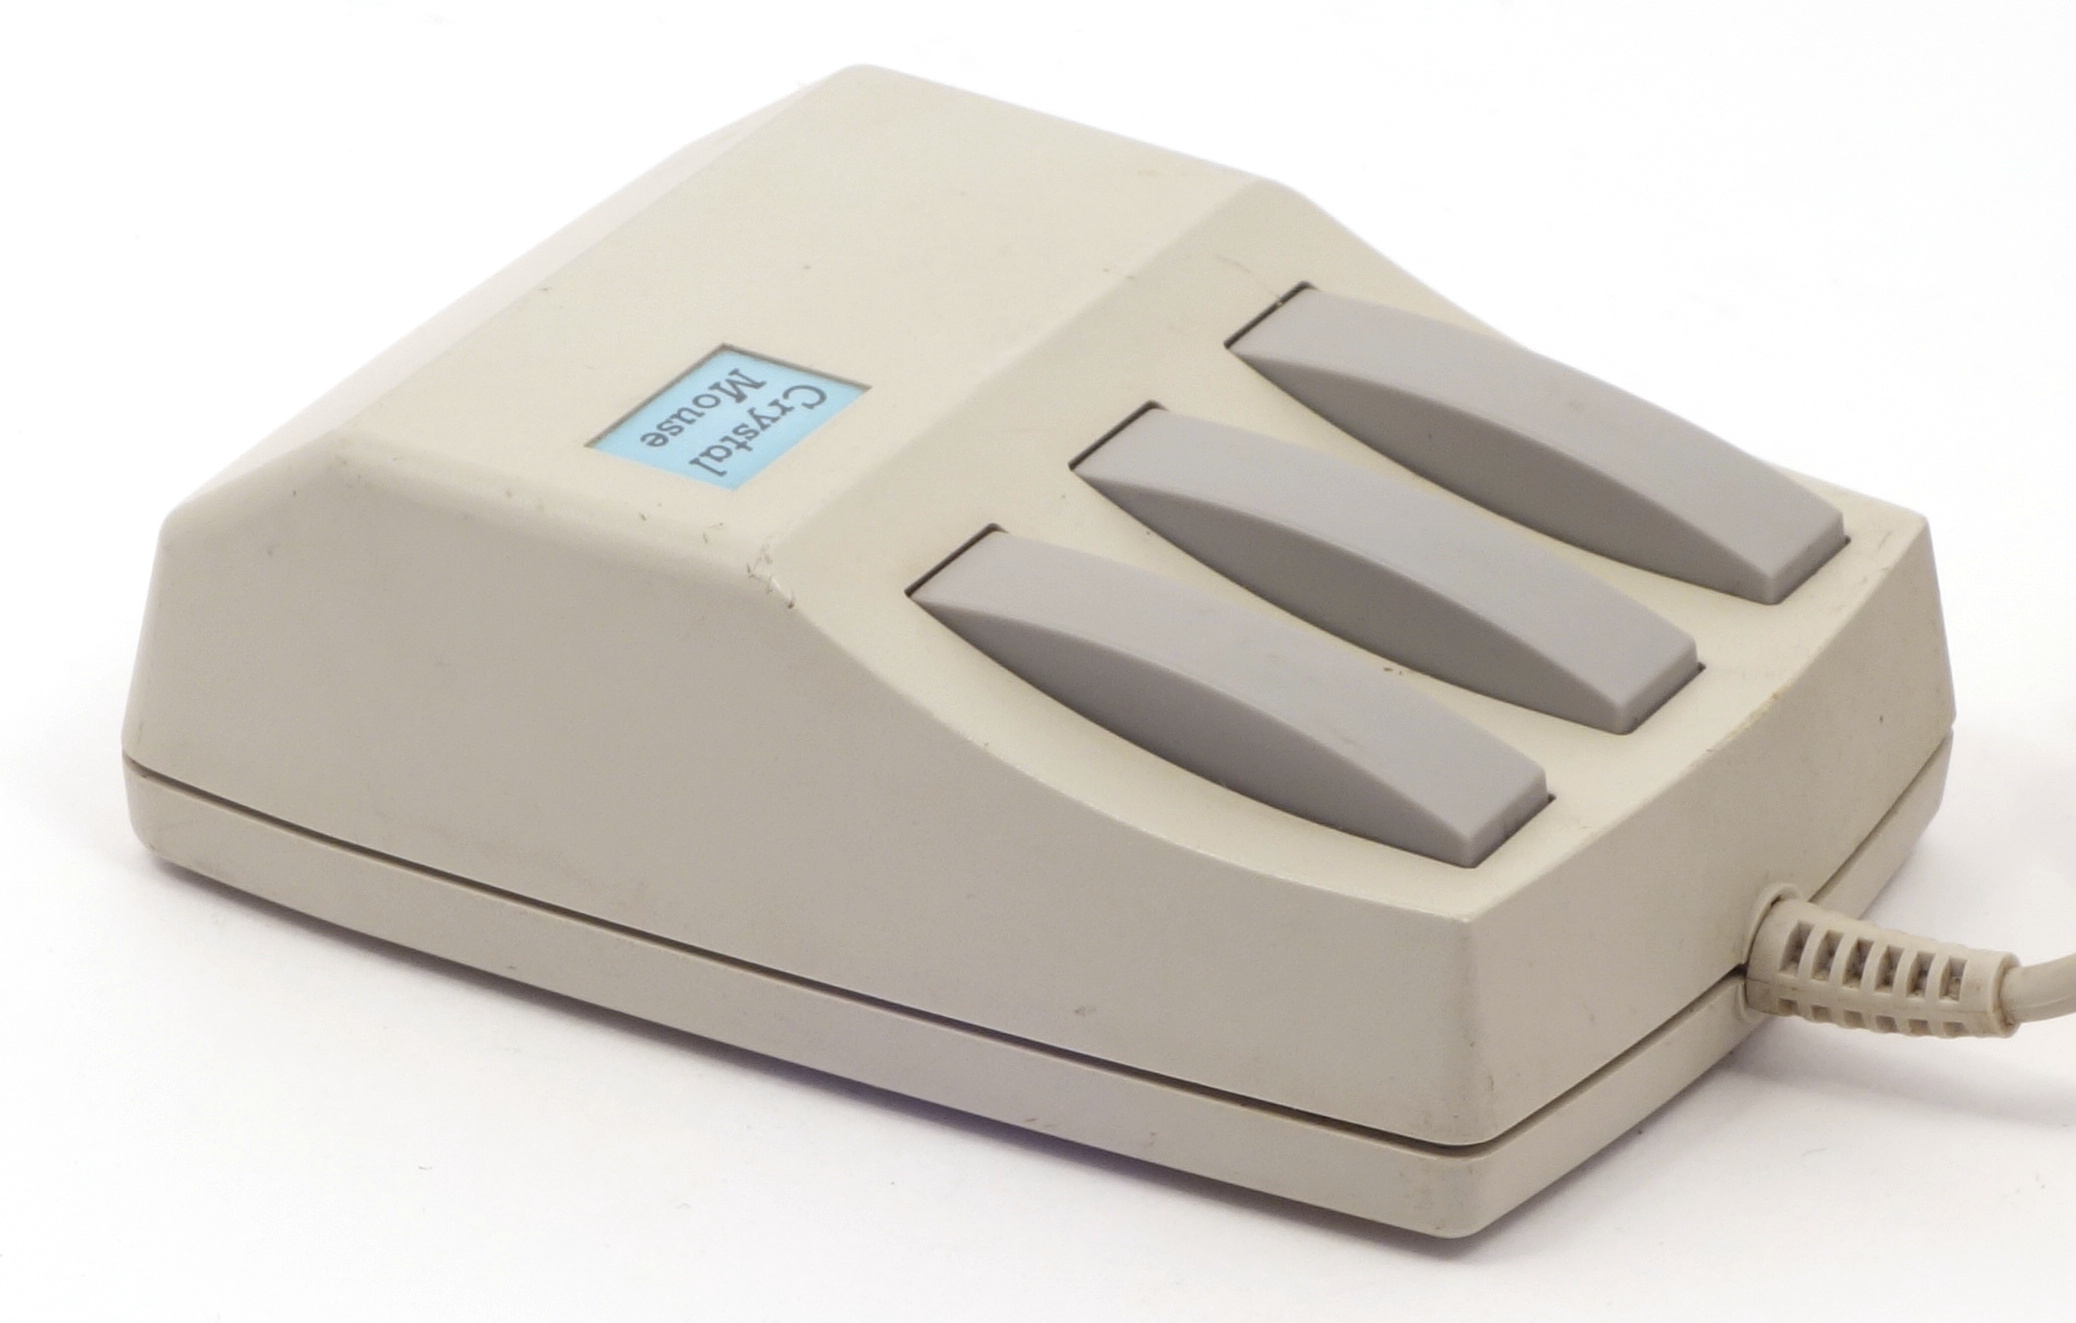
\includegraphics[scale=0.7]{1986_nec_crystal_mouse/necNorm_30.jpg}
    \caption{NEC Crystal Mouse}
    \label{fig:NECCrystalPic}
\end{figure}

The name of the mouse “Crystal Mouse” is highlighted on the upper side of the case with two triangular stylized mice in outlines and solid lines. The bottom side shows that this is an optical mouse (figure \ref{NecCrystalTopAndBottom}), which largely repeats the external design solutions of the Mouse Systems mice of the same period and is intended for use with a special mirror pad \cite{photo}.

\begin{figure}[h]
    \centering
    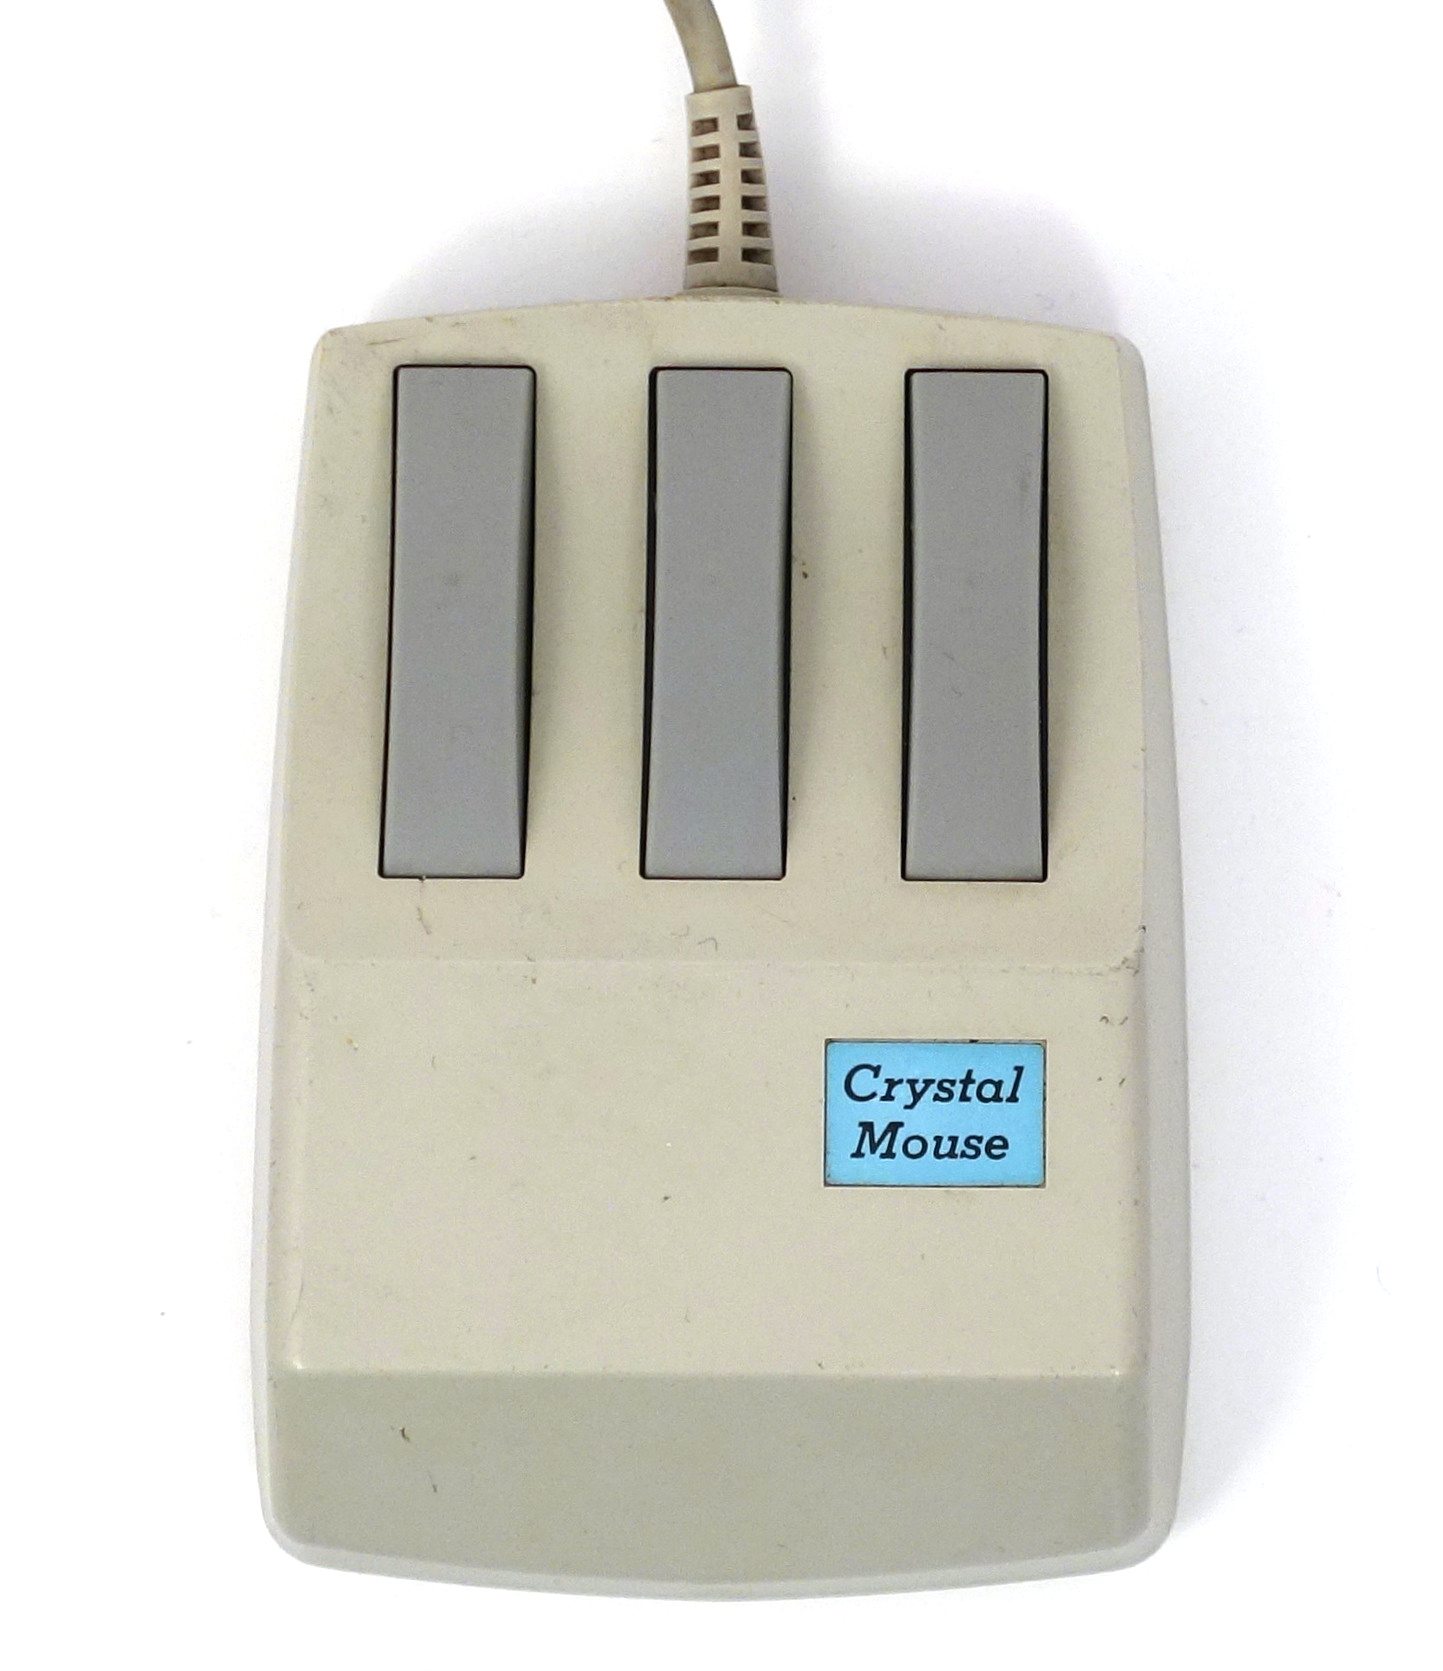
\includegraphics[scale=0.5]{1986_nec_crystal_mouse/nectop_60.jpg}
    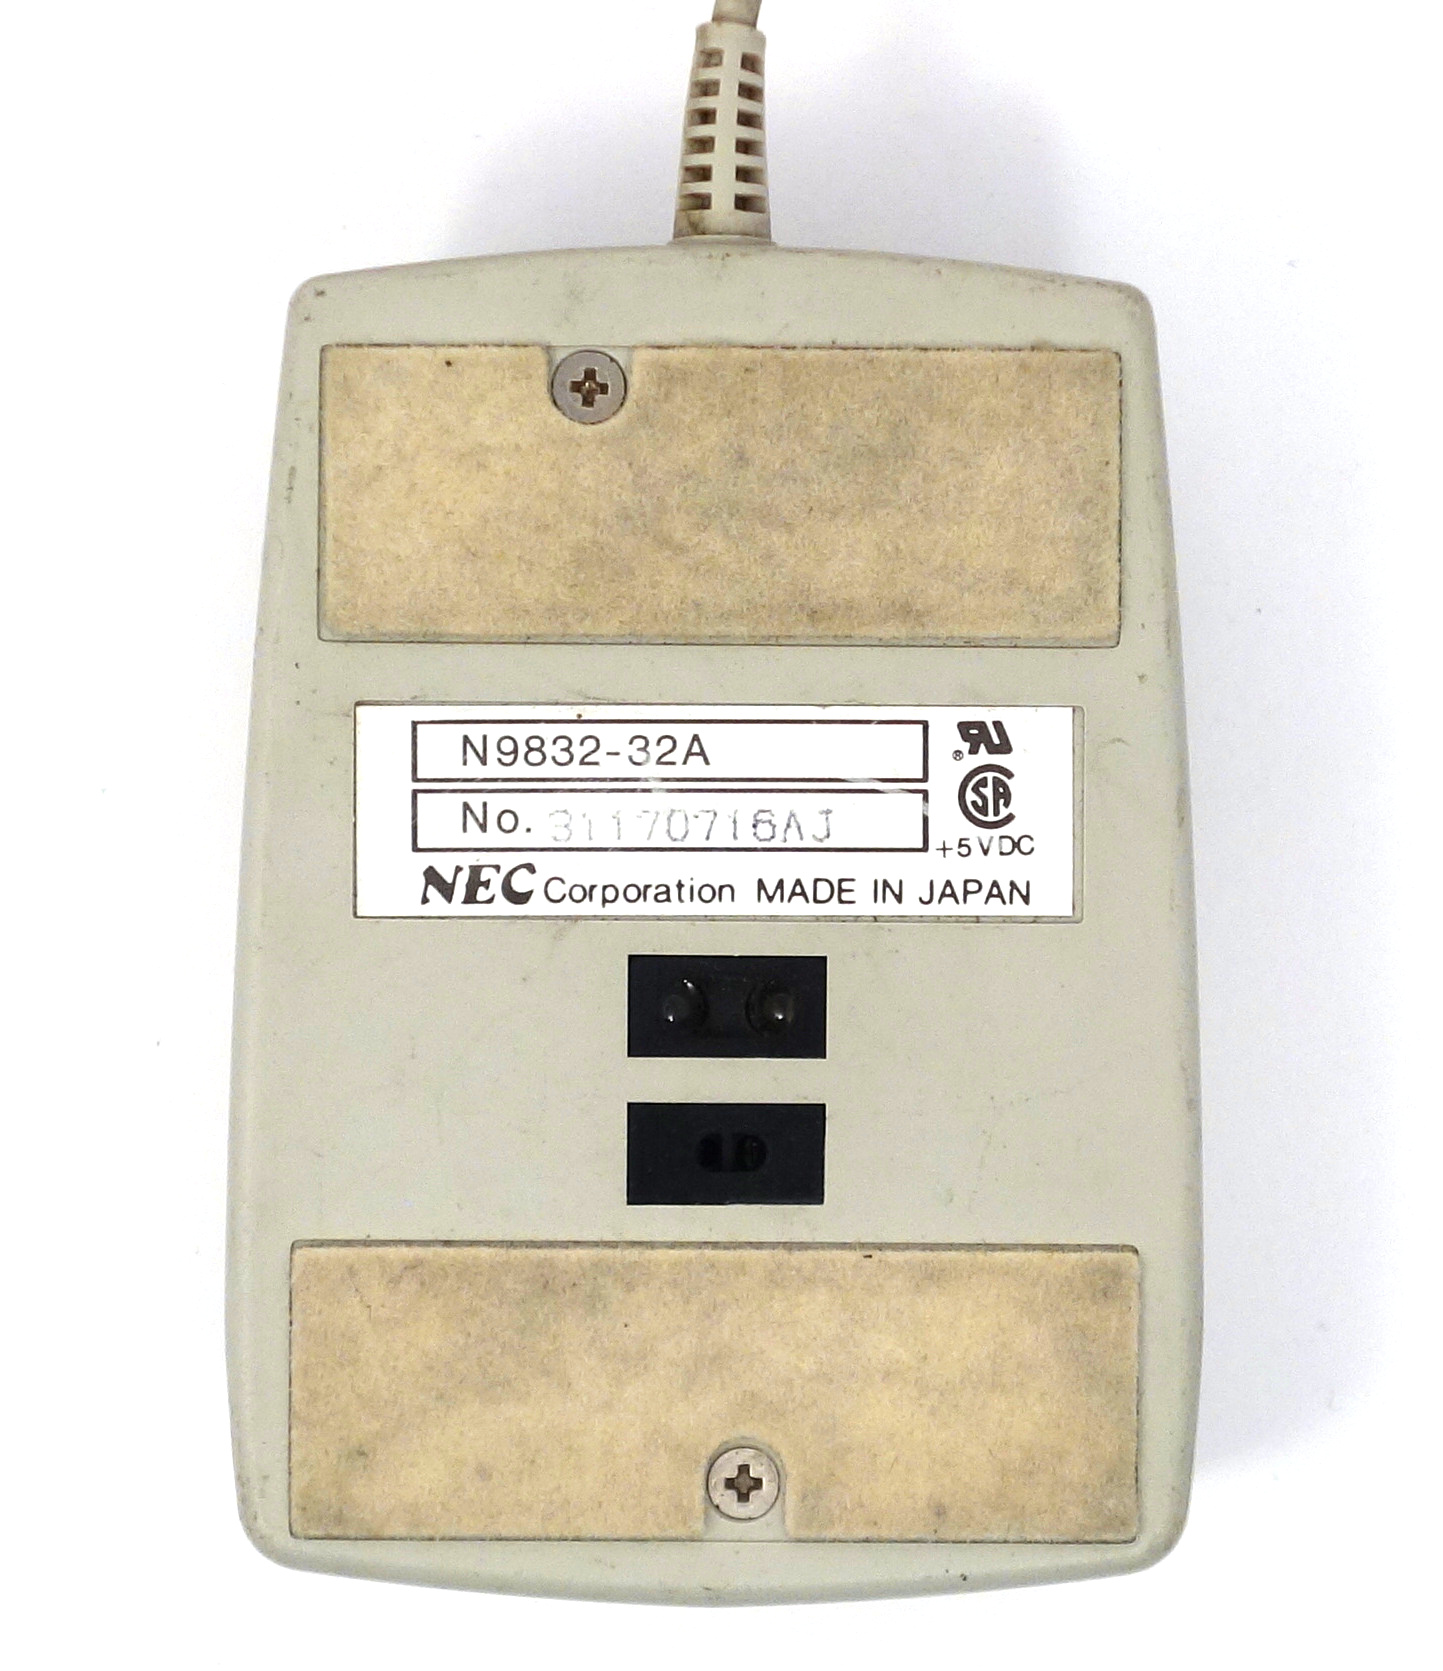
\includegraphics[scale=0.5]{1986_nec_crystal_mouse/necbottom_60.jpg}
    \caption{NEC Crystal Mouse, top and bottom views}
    \label{NecCrystalTopAndBottom}
\end{figure}

In terms of size, the manipulator is an optical cursor control device typical for the 80s (figure \ref{fig:NecCrystalSize}).

\begin{figure}[h]
    \centering
    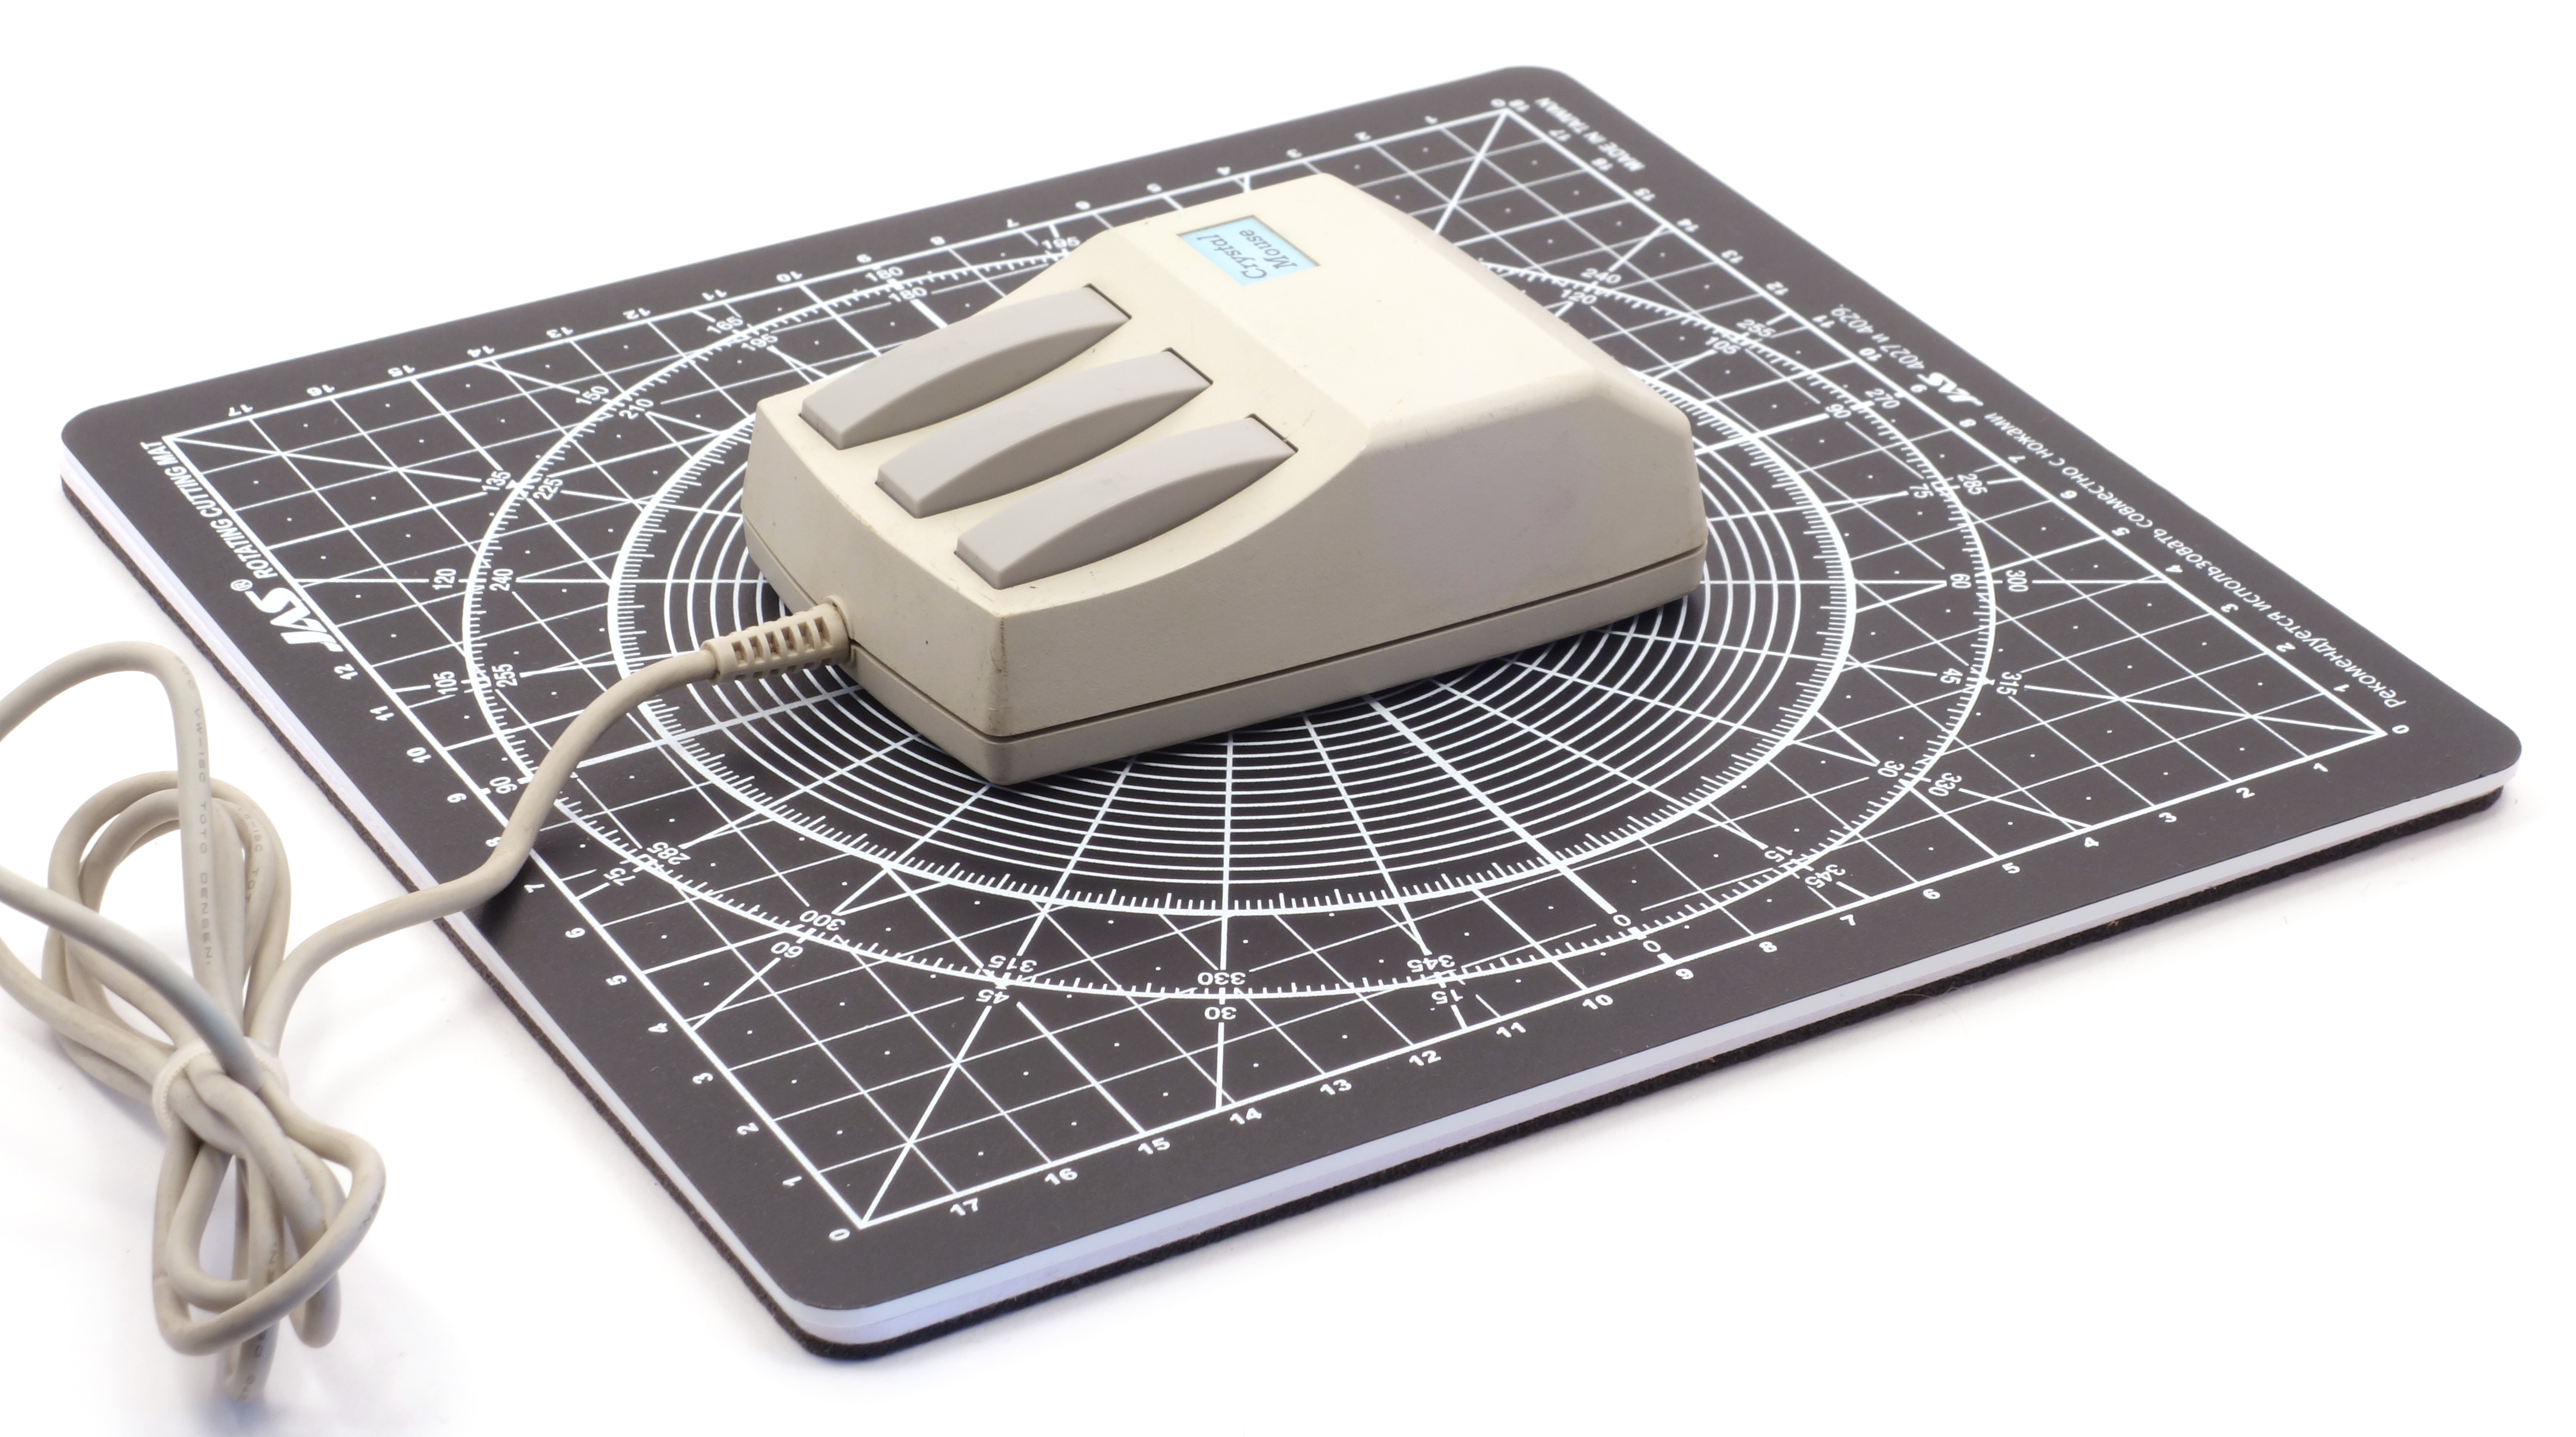
\includegraphics[scale=0.4]{1986_nec_crystal_mouse/NecKovrik_60.jpg}
    \caption{NEC Crystal Mouse on a graduated pad with a grid step of 1~cm}
    \label{fig:NecCrystalSize}
\end{figure}

In terms of ergonomics, the exterior of the Crystal Mouse has a strong industrial design. At the same time, a large number of corners and flat edges are partly compensated by rounded joints of the edges in the part of the body closest to the user and convex long buttons conveniently located within the reach of the fingers (figure \ref{fig:NecCrystalHand}).

\begin{figure}[h]
    \centering
    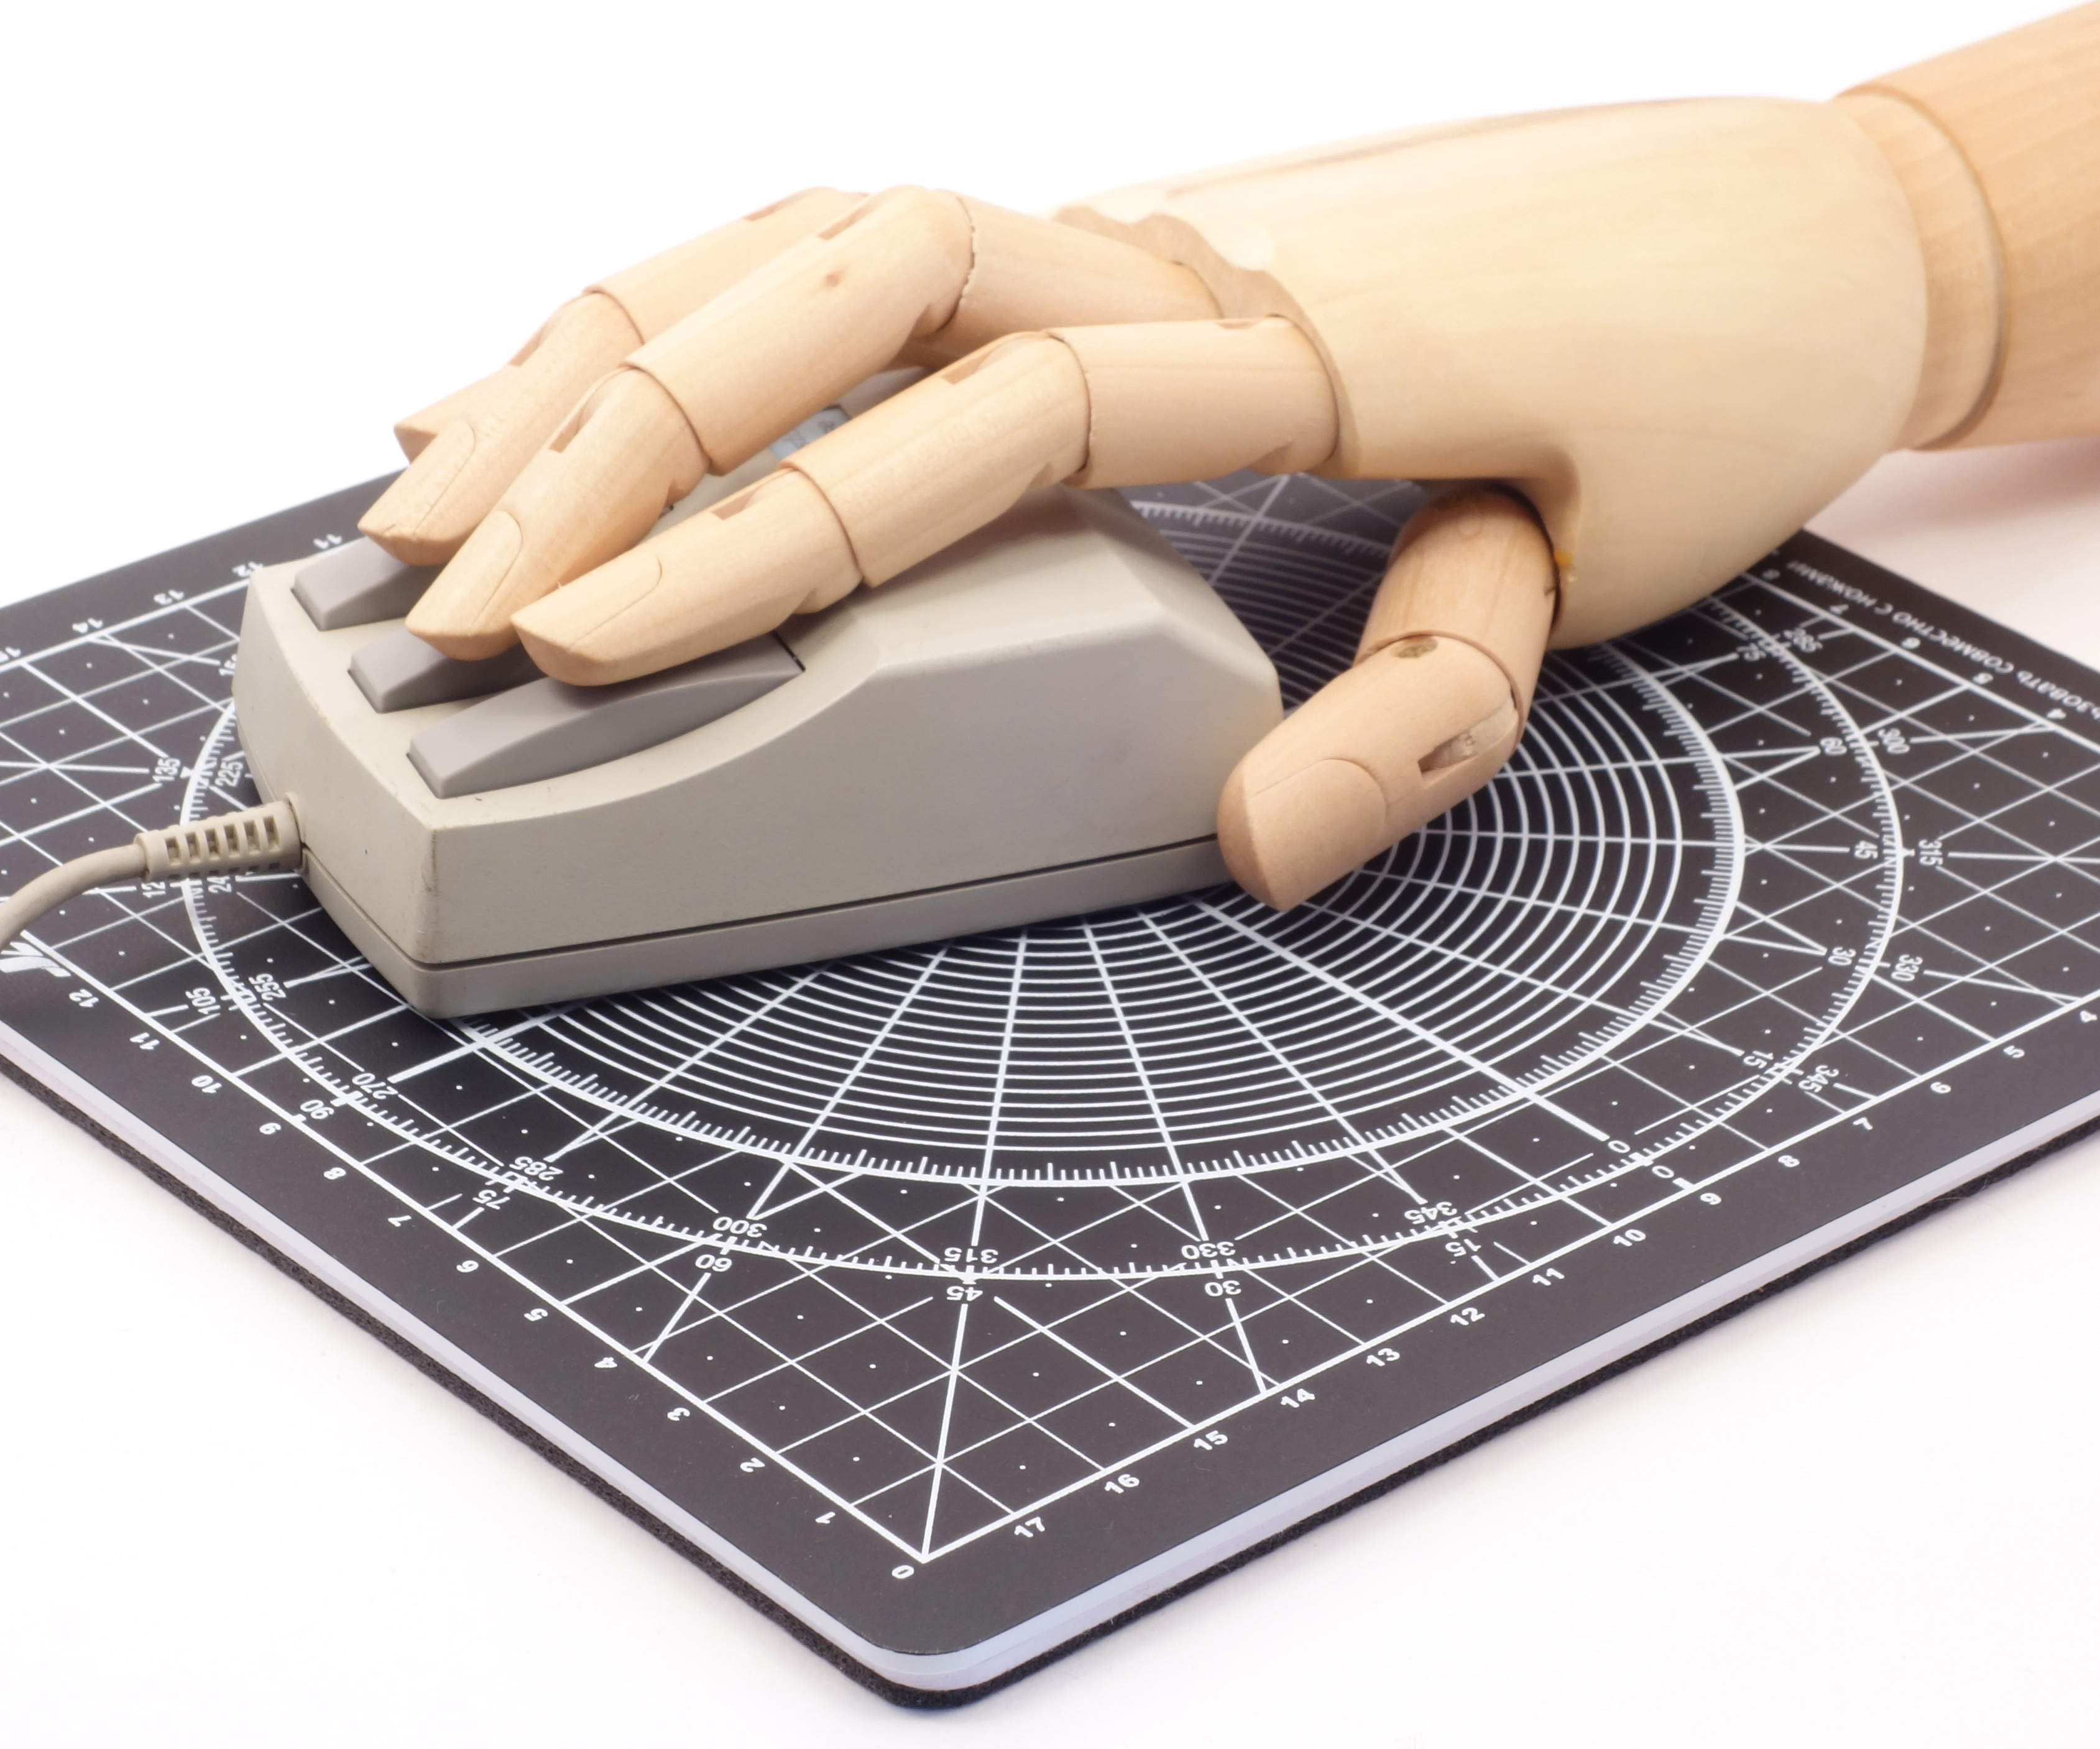
\includegraphics[scale=0.4]{1986_nec_crystal_mouse/NecRuka_30.jpg}
    \caption{NEC Crystal Mouse with a human hand model}
    \label{fig:NecCrystalHand}
\end{figure}

NEC Crystal Mouse has a DIN connector and belongs to the Bus Mouse category according to the connection interface. A feature of such mice is that the optocoupler signals are processed not by a chip in the mouse case, but by a special adapter in the computer system unit; therefore, this mouse is powered by the computer without a separate power supply, unlike many early optical models that were connected to the serial port of the IBM PC.

\begin{figure}[h]
    \centering
    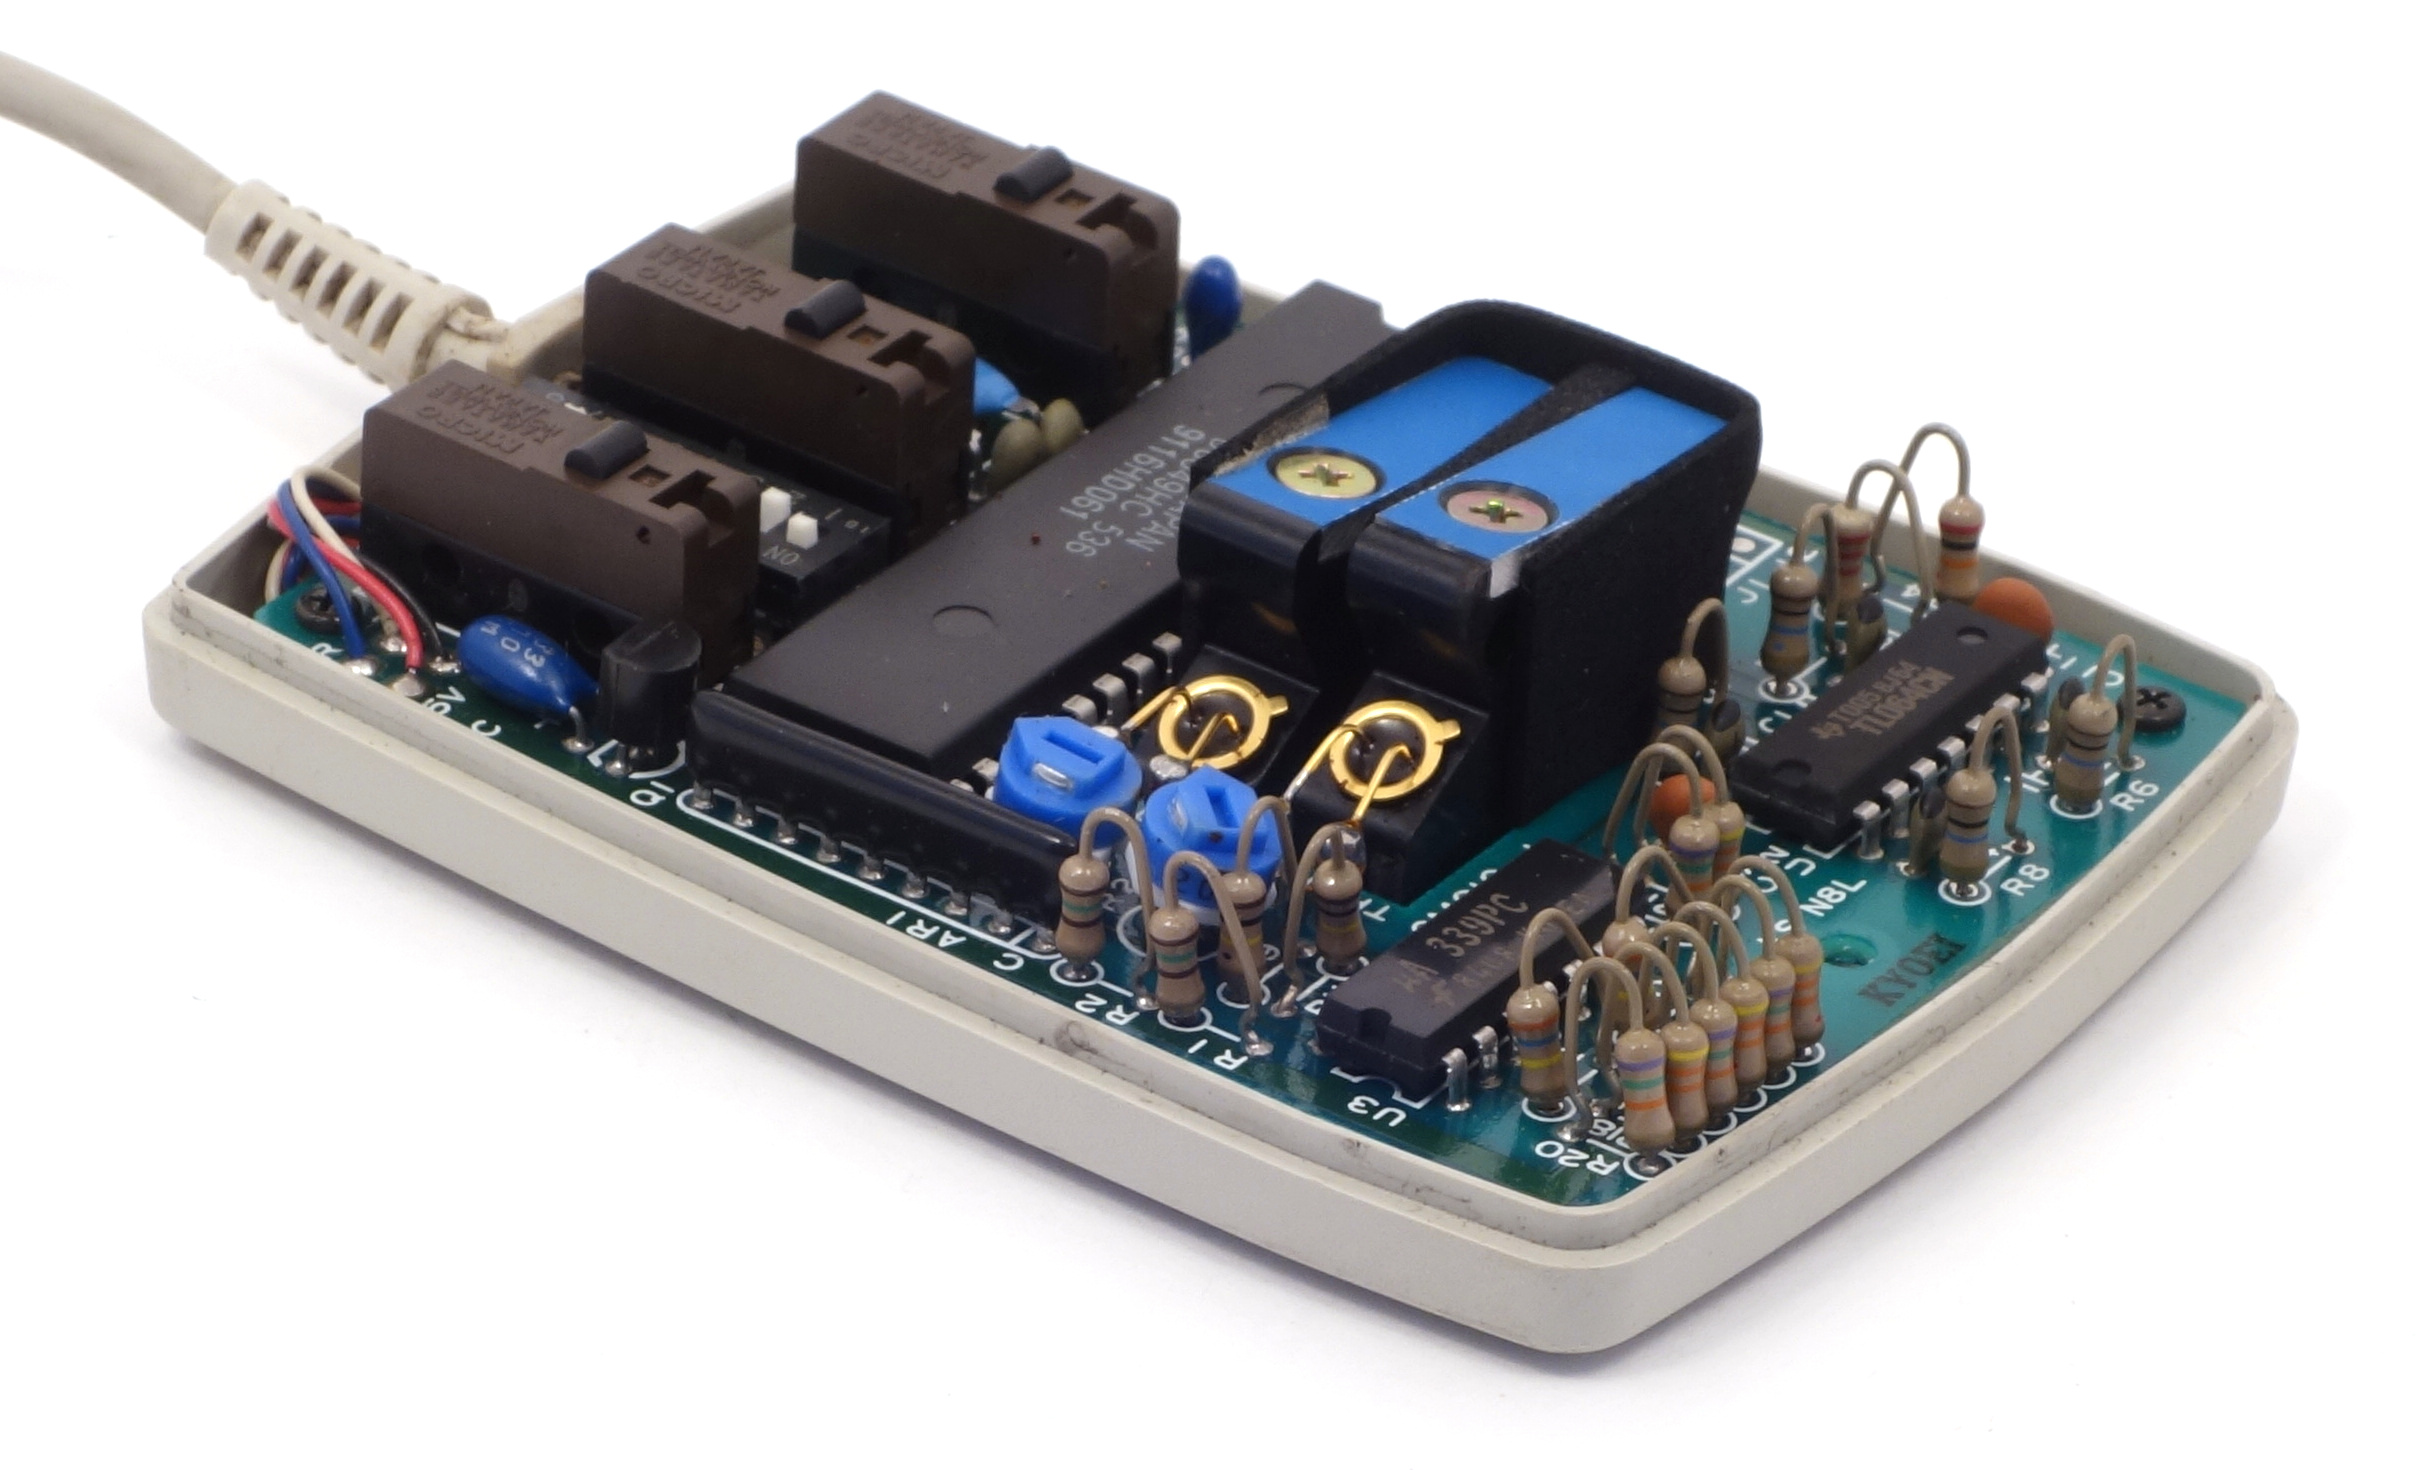
\includegraphics[scale=0.8]{1986_nec_crystal_mouse/necraz_60.jpg}
    \caption{NEC Crystal Mouse disassembled}
    \label{fig:NecCrystalInside}
\end{figure}

Mouse internals are shown on figure \ref{fig:NecCrystalInside}. You can see the original design of this optical mouse. Unlike most optical mice of the 80s, it is not a direct copy of the Mouse Systems device, which has become a prototype for subsequent manipulators of this type.

\begin{thebibliography}{9}
\bibitem {yt} NEC EWS4800 \url{http://museum.ipsj.or.jp/en/computer/work/0003.html}
\bibitem {photo} Graphics NEC EWS4800 \url{http://www.cs.ce.nihon-u.ac.jp/facility/exp-gazo.html}
\end{thebibliography}
\end{document}
